\section{Introduction} \label{s:intro}

% \TODO{
% This section includes the context and motivation behind the work, explicitly or implicitly highlights the main research question(s), provides a high-level explanation of the solution, and describes the contributions.}

% \TODO{Context, motivation, research question asds, and original contribution could be organized in subsections.}




% \begin{figure}[!h]
%     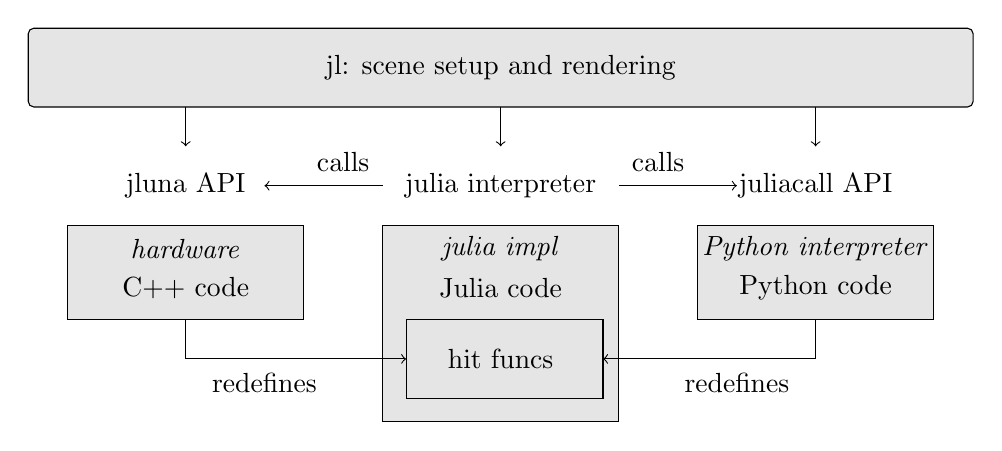
\begin{tikzpicture}
  % beveled 10x4 rectangle with text in the middle "jl: scene setup and rendering"
  \draw[rounded corners=2pt, fill=black!10] (0,0) rectangle (12,1);
  \node at (6,0.5) {jl: scene setup and rendering};
  % arrow down 2 units @ (1.5, 1)
  \draw[->] (2,0) -- (2,-.5);
  \node at (2,-1) {jluna API};
  % draw box 3 wide and 2 tall below node 
  \draw[fill=black!10] (.5,-1.5) rectangle (3.5,-2.7);
  % draw text at top of this box in italics "hardware"
  \node at (2,-1.8) {\textit{hardware}};
  \node at (2, -2.3) {C++ code};
  
  \draw[fill=black!10] (4.5,-1.5) rectangle (7.5,-4);
  \node at (6,-1.8) {\textit{julia impl}};
  \node at (6, -2.3) {Julia code};
  % draw box inside julia code box and inside that write "hit funcs"
  \draw[fill=black!10] (4.8,-2.7) rectangle (7.3,-3.7);
  \node at (6,-3.2) {hit funcs};
  
  % arrow that bends 90 degrees into julia impl from bottom of c++ box 
  \draw[->] (2,-2.7) -- (2,-3.2) -- (4.8,-3.2);
  % add text below arrow that says "redefines"
  \node at (3,-3.5) {redefines};

  % arrow down 2 units @ (7.5, 1)
  \draw[->] (10,0) -- (10,-.5);
  \node at (10,-1) {juliacall API};
  % draw box 3 wide and 2 tall below node
  \draw[fill=black!10] (8.5,-1.5) rectangle (11.5,-2.7);
  % draw text at top of this box in italics "julia impl"
  \node at (10,-1.8) {\textit{Python interpreter}};
  \node at (10, -2.3) {Python code};
  
  % arrow that bends 90 degrees into julia impl from bottom of python box
  \draw[->] (10,-2.7) -- (10,-3.2) -- (7.3,-3.2);
  % add text below arrow that says "redefines"
  \node at (9,-3.5) {redefines};

  % arrow down in the middle between above 2 
  \draw[->] (6,0) -- (6, -.5);
  \node at (6,-1) {julia interpreter};
  % arrow from julia interpreter to jluna API with the text "calls"
  \draw[->] (4.5,-1) -- (3, -1);
  \node at (4,-.7) {calls};

  % arrow from julia interpreter to juliacall API with the text "calls"
  \draw[->] (7.5,-1) -- (9, -1);
  \node at (8,-.7) {calls};
\end{tikzpicture}

% \end{figure}

% briefly talk about physically based rendering 
Computational ray tracing and more broadly physically based rendering developed its theoretical foundation in the mid to late 20th century. As hardware improved the viability and practicality of ray tracing in various domains became more common. Alongside the improvements in hardware came the development ray-tracing specific hardware, more commonly known as application-specific integrated circuits or ASICs for short. These ASICs were specifically designed to accelerate common patterns in ray-tracing operations. Ray tracing ASICs where intially a largely academic pursuit from around the mid 90s to the early 2010s. In 2018 Nvidia announced its Turing architecture which included the first consumer-grade ray tracing ASIC, the RT core. 

The introduction of the RT core in consumer-grade hardware marked a significant shift in the industry. Ray tracing was no longer a niche technology but readily available to the average consumer. Which in turn meant that applications of ray tracing could now be more widely adopted. A key area being the videogame industry. However with this wider adoption, especially for videogames came an increased focus on performance and optimizations.

% talk about the relevance of performance and optimizations 

% talk about the motivation behind the comparative analysis
    % what is the general idea behind the analysis
    % what are the goals of the analysis
    % what are the expected outcomes of the analysis
    % what isthe importance of this

% give some of the research questions that will be answered in the analysis

% give a brief overview of the methodology used in the analysis




% ---------- templates for figures ----------------------- 

% \begin{figure}[bh]
%     %% The macro `\onecolgrid' is defined in `vusec.sty'
%     %% NOTE: The suffix "./figures/" is implicitly included for this relative path.
%     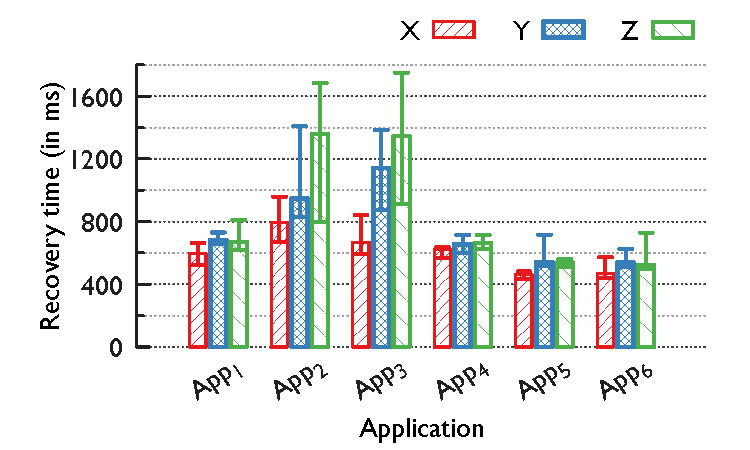
\includegraphics[width=\onecolgrid]{cache-by-app}
%     %% Labels should immediately follow caption, to keep latex quiet.
%     \figcap{Simple one-column figure. Please include a brief explanation or takeaway.}\label{fig:1col}
% \end{figure}

% \begin{figure*}[th]
%     %% The macro `\threecolgrid' is defined in `vusec.sty'
%     \begin{subfigure}[t]{\threecolgrid}
%         %% NOTE: The suffix "./figures/" is implicitly included for these relative paths.
%         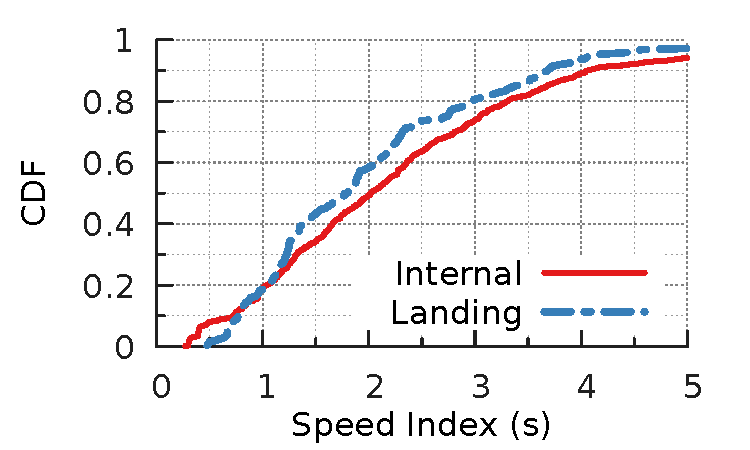
\includegraphics[width=\linewidth]{three-col/speed_index}
%         \sfigcap{}\label{fig:3col-a}
%     \end{subfigure}
%     \begin{subfigure}[t]{\threecolgrid}
%         %% NOTE: You do not have to mention the extension.
%         %% (The example figures are in PDF format.)
%         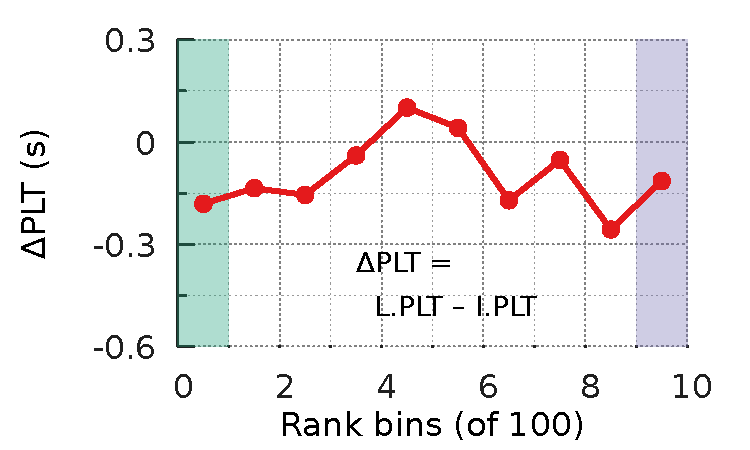
\includegraphics[width=\linewidth]{three-col/plt_ranks_diff}
%         \sfigcap{}\label{fig:3col-b}
%     \end{subfigure}
%     \begin{subfigure}[t]{\threecolgrid}
%         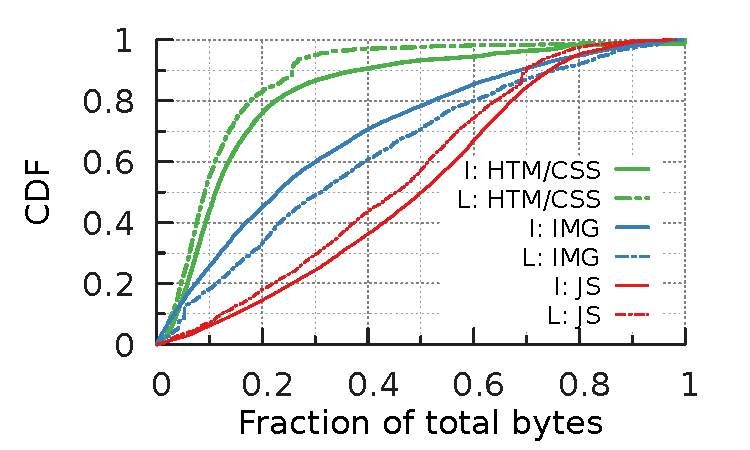
\includegraphics[width=\linewidth]{three-col/mimes}
%         \sfigcap{}\label{fig:3col-c}
%     \end{subfigure}
%     %% Labels should immediately follow caption, to keep latex quiet.
%     \figcap{Generate clear and beautiful figures (in PDF) that can be rendered side by side while still being easy to read and interpret. Choose colors wisely from the colorbrewer2.org website.}\label{fig:3col}
% \end{figure*}

% \begin{table}[hb]
%     \centering
%     \tabcap{A simple table describing the characteristics of a data set or the results of an experiment}\label{tab:sample}
%     \taburulecolor{black!45}
%     \begin{tabu}{c|c|r|r|r|r}
%         \toprule
%         \multirow{2}{*}{\thead{Char.}} &
%             \multirow{2}{*}{\thead{\#samples}} &
%             \thead{Count} &
%             \multicolumn{3}{c}{\thead{Perf. Score}}\\
%         &
%             &
%             \thead{of items} &
%             \thead{X} & \thead{Y} & \thead{Z} \\
%         \midrule
%         \stress{P}
%             & 214 & 56 & 9 & 23 & 24 \\
%         \stress{Q}
%             & 117 & 27 & 7 & 10 & 10 \\
%         \stress{R}
%             & 222 & 11 & 6 & 4 & 1 \\
%         \stress{S}
%             & 187 &  9 & 1 & 6 & 2 \\
%         \stress{T}
%             & 180 & 16 & 7 & 5 & 4 \\
%         \bottomrule
%     \end{tabu}

% \end{table}

 